\section{eo\-Ranking\-Select$<$ EOT $>$ Class Template Reference}
\label{classeo_ranking_select}\index{eoRankingSelect@{eoRankingSelect}}
eo\-Ranking\-Select: select an individual by roulette wheel on its rank is an {\bf eo\-Roulette\-Worth\-Select}{\rm (p.\,\pageref{classeo_roulette_worth_select})}, i.e.  


{\tt \#include $<$eo\-Ranking\-Select.h$>$}

Inheritance diagram for eo\-Ranking\-Select$<$ EOT $>$::\begin{figure}[H]
\begin{center}
\leavevmode
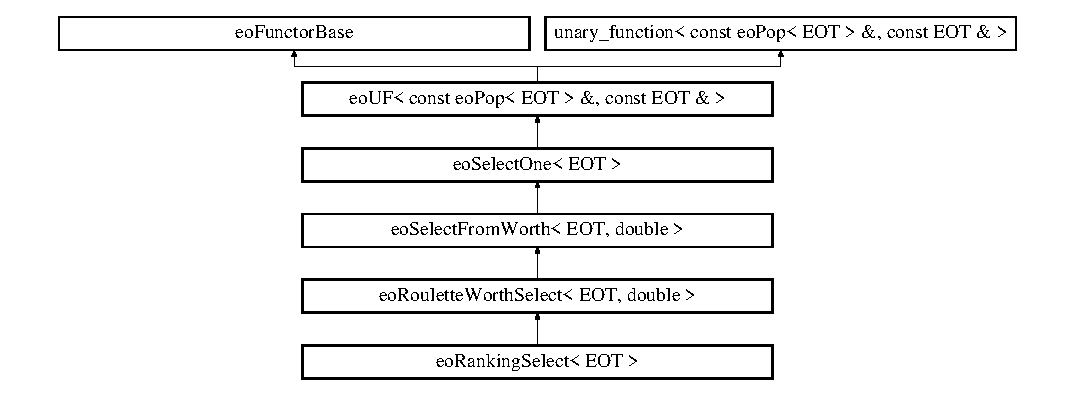
\includegraphics[height=4.85549cm]{classeo_ranking_select}
\end{center}
\end{figure}
\subsection*{Public Member Functions}
\begin{CompactItemize}
\item 
{\bf eo\-Ranking\-Select} (double \_\-p=2.0, double \_\-e=1.0)
\begin{CompactList}\small\item\em Ctor:. \item\end{CompactList}\end{CompactItemize}
\subsection*{Private Attributes}
\begin{CompactItemize}
\item 
{\bf eo\-Ranking}$<$ {\bf EOT} $>$ {\bf ranking}\label{classeo_ranking_select_r0}

\end{CompactItemize}


\subsection{Detailed Description}
\subsubsection*{template$<$class EOT$>$ class eo\-Ranking\-Select$<$ EOT $>$}

eo\-Ranking\-Select: select an individual by roulette wheel on its rank is an {\bf eo\-Roulette\-Worth\-Select}{\rm (p.\,\pageref{classeo_roulette_worth_select})}, i.e. 

a selector using a std::vector of worthes rather than the raw fitness (see {\bf eo\-Select\-From\-Worth.h}{\rm (p.\,\pageref{eo_select_from_worth_8h})}) uses an internal {\bf eo\-Ranking}{\rm (p.\,\pageref{classeo_ranking})} object which is an {\bf eo\-Perf2Worth$<$EOT, double$>$}{\rm (p.\,\pageref{classeo_perf2_worth})} 



Definition at line 41 of file eo\-Ranking\-Select.h.

\subsection{Constructor \& Destructor Documentation}
\index{eoRankingSelect@{eo\-Ranking\-Select}!eoRankingSelect@{eoRankingSelect}}
\index{eoRankingSelect@{eoRankingSelect}!eoRankingSelect@{eo\-Ranking\-Select}}
\subsubsection{\setlength{\rightskip}{0pt plus 5cm}template$<$class EOT$>$ {\bf eo\-Ranking\-Select}$<$ {\bf EOT} $>$::{\bf eo\-Ranking\-Select} (double {\em \_\-p} = {\tt 2.0}, double {\em \_\-e} = {\tt 1.0})\hspace{0.3cm}{\tt  [inline]}}\label{classeo_ranking_select_a0}


Ctor:. 

\begin{Desc}
\item[Parameters:]
\begin{description}
\item[{\em \_\-p}]the selective pressure, should be in [1,2] (2 is the default) \item[{\em \_\-e}]exponent (1 == linear) \end{description}
\end{Desc}


Definition at line 48 of file eo\-Ranking\-Select.h.

The documentation for this class was generated from the following file:\begin{CompactItemize}
\item 
eo\-Ranking\-Select.h\end{CompactItemize}
